\documentclass{article}
\usepackage[margin=0.7in]{geometry}
\usepackage[parfill]{parskip}
\usepackage[utf8]{inputenc}
\usepackage[lithuanian]{babel}
\usepackage[T1]{fontenc}
\usepackage{amsmath,amssymb,amsfonts,amsthm}
\usepackage{tikz}

\title{6 Uždavinys}
\author{Arnas Vaicekauskas}

\begin{document}

\maketitle

\section{Matematinis modelis}

\subsection{Bedimensis modelis}

\begin{subequations} \label{nodim}
    \begin{align}
    \frac{\partial c_1}{\partial t}&=-3c_1c_2+D\Delta c_1\\
    \frac{\partial c_2}{\partial t}&=-5c_1c_2+D\Delta c_2\\
    \frac{\partial c_3}{\partial t}&=2c_1c_2
    \end{align}
\end{subequations}

kur $c_1,c_2,c_3$ yra bedimensė medžiagų koncentracija, 
$\Delta$ - Laplaso operatorius, $t$ - laikas, 
$D$ - bedimensis medžiagų $c_1$ ir $c_2$ difuzijos koeficientas.

\subsection{Elementų maišymasis dviejose dimensijose}

Interpretavus bedimensį modelį \eqref{nodim} dviejose dimensijose gauname lygtis

\begin{subequations} \label{rect}
    \begin{align}
    \frac{\partial c_1}{\partial t}&=-3c_1c_2+D\left(\frac{\partial^2c_1}{\partial x^2}+\frac{\partial^2c_1}{\partial y^2}\right)\\
    \frac{\partial c_2}{\partial t}&=-5c_1c_2+D\left(\frac{\partial^2c_2}{\partial x^2}+\frac{\partial^2c_2}{\partial y^2}\right)\\
    \frac{\partial c_3}{\partial t}&=2c_1c_2
    \end{align}
\end{subequations}

Šiam modeliui yra taikomos šios pradinės ir kraštinės sąlygos:

\begin{align*} \label{2d-init-cond}
    \frac{\partial c_1}{\partial x}\Big|_{x=0}&=\frac{\partial c_1}{\partial x}\Big|_{x=L}=\frac{\partial c_2}{\partial x}\Big|_{x=0}=\frac{\partial c_2}{\partial x}\Big|_{x=L}=0, &y&\in[0,L], t\in[0,T]\\
    \frac{\partial c_1}{\partial y}\Big|_{y=0}&=\frac{\partial c_1}{\partial y}\Big|_{y=L}=\frac{\partial c_2}{\partial y}\Big|_{y=0}=\frac{\partial c_2}{\partial y}\Big|_{y=L}=0, &x&\in[0,L], t\in[0,T]\\
    c_1(x, y, 0) &= 
    \begin{cases}
        1, \text{jei } x\in A\\
        0, \text{kitaip}
    \end{cases}
    c_2(x, y, 0) = 
    \begin{cases}
        1, \text{jei } x\notin A\\
        0, \text{kitaip}
    \end{cases},&(x, y)&\in[0,L]^2, A=\left[0, \tfrac{L}{2}\right]^2\cup\left[\tfrac{L}{2},L\right]^2\\
    c_3(x, y, 0) &= 0,&(x, y)&\in[0,L]^2,
\end{align*}

kur $L$ - bedimensis kubo kraštinės ilgis, $T$ - bedimensė proceso trukmė.

\begin{figure}[h!]
    \centering
    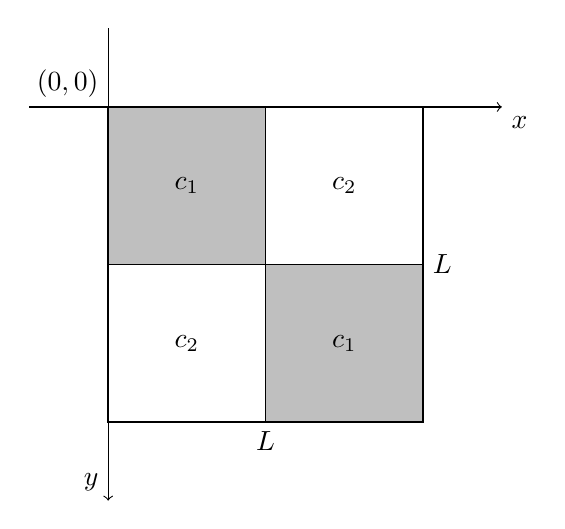
\begin{tikzpicture}[scale=2.0]
        \draw[fill=white] (0,0) rectangle (1,1);
        \draw[fill=white] (1,1) rectangle (2,2);
        \draw[fill=gray!50] (0,1) rectangle (1,2);
        \draw[fill=gray!50] (1,0) rectangle (2,1);
        
        % Draw the boundary of the square
        \draw[thick] (0,0) rectangle (2,2);
    
        % Draw axes
        \draw[->] (-0.5,2) -- (2.5,2) node[anchor=north west] {$x$};  % x-axis
        \draw[<-] (0,-0.5) node[anchor=south east] {$y$} -- (0,2.5);  % y-axis
    
        % Mark the origin
        \node[anchor=south east] at (0,2) {$(0, 0)$};
        
        % Mark the side length L
        \draw[-] (2,0) -- (2,2) node[midway, right] {$L$};
        \draw[-] (0,0) -- (2,0) node[midway, below] {$L$};
        \draw (0.5, 1.5) node[anchor=center] {$c_1$};
        \draw (1.5, 0.5) node[anchor=center] {$c_1$};
        \draw (1.5, 1.5) node[anchor=center] {$c_2$};
        \draw (0.5, 0.5) node[anchor=center] {$c_2$};
    \end{tikzpicture}
    \caption{Dvimačio modelio pradinės sąlygos laiku $t=0$. Pilka spalva žymi plotą priklausantį aibei $A$. }
\end{figure}

\newpage
\section{Skaitiniai modeliai}

Remiantis išreikštiniu baigtinių skirtumų metodu iš dvimačio modelio galima gauti skaitinį modelį.
\begin{subequations} \label{numerical-eqs}
\begin{align}
\frac{c^{n+1}_{1,i,j}-c^n_{1,i,j}}{\Delta t}&=
-3c^{n}_{1,i,j}c^{n}_{2,i,j}
+D\left(\frac{c^n_{1,i-1,j}-2c^n_{1,i,j}+c^n_{1,i+1,j}}{(\Delta x)^2}+\frac{c^n_{1,i,j-1}-2c^n_{1,i,j}+c^n_{1,i,j+1}}{(\Delta y)^2}\right)\\
\frac{c^{n+1}_{2,i,j}-c^n_{2,i,j}}{\Delta t}&=
-5c^{n}_{1,i,j}c^{n}_{2,i,j}
+D\left(\frac{c^n_{2,i-1,j}-2c^n_{2,i,j}+c^n_{2,i+1,j}}{(\Delta x)^2}+\frac{c^n_{2,i,j-1}-2c^n_{2,i,j}+c^n_{2,i,j+1}}{(\Delta y)^2}\right)\\
\frac{c^{n+1}_{3,i,j}-c^n_{3,i,j}}{\Delta t}&=2c^{n}_{1,i,j}c^{n}_{2,i,j},
\end{align}
\end{subequations}

kur $n\in[0, T)$ - laiko momentas, 
$i\in[0,N_L)$ - diskrečios erdvės taško koordinatė $x$ ašyje,
$j\in[0,N_L)$ - diskrečios erdvės taško koordinatė $y$ ašyje,
$c^n_{1,i,j}$ - pirmos medžiagos kiekis diskrečios erdvės taške $i$, $j$ laiko momentu $n$,
$c^n_{2,i,j}$ - antros medžiagos kiekis diskrečios erdvės taške $i$, $j$ laiko momentu $n$,
$c^n_{3,i,j}$ - trečios medžiagos kiekis diskrečios erdvės taške $i$, $j$ laiko momentu $n$,
$\Delta t$ - laiko žingsnis,
$\Delta x$ - diskrečios erdvės žingsnis $x$ ašimi,
$\Delta y$ - diskrečios erdvės žingsnis $y$ ašimi.

\newpage
\subsubsection{Laiko žingsnio pasirinkimas}

Pertvarkius skaitinio modelio lygtis \eqref{numerical-eqs} taip, kad kairėje lygties pusėje liktų 
medžiagos kiekis sekančiu laiko momentu ir sugrupavus pastovius narius pagal medžiagos kiekio
praėjusį laiko momentą gauname išraiška koeficiento, kuris nusako kiek medžiagos
ląstelėje $i,j$ persikels į sekantį laiko momentą.     

\begin{subequations}
    \begin{align}
    c^{n+1}_{1,i,j}&=
    \left(1-\Delta t\left(3c^{n}_{2,i,j}+2D\left(\frac{1}{(\Delta x)^2}+\frac{1}{(\Delta y)^2}\right)\right)\right)c^n_{1,i,j}
    +D\Delta t\left(\frac{c^n_{1,i-1,j}+c^n_{1,i+1,j}}{(\Delta x)^2}+\frac{c^n_{1,i,j-1}+c^n_{1,i,j+1}}{(\Delta y)^2}\right)\\
    c^{n+1}_{2,i,j}&=
    \left(1-\Delta t\left(5c^{n}_{1,i,j}+2D\left(\frac{1}{(\Delta x)^2}+\frac{1}{(\Delta y)^2}\right)\right)\right)c^n_{2,i,j}
    +D\Delta t\left(\frac{c^n_{2,i-1,j}+c^n_{2,i+1,j}}{(\Delta x)^2}+\frac{c^n_{2,i,j-1}+c^n_{2,i,j+1}}{(\Delta y)^2}\right)\\
    c^{n+1}_{3,i,j}&=c^n_{3,i,j}+2\Delta tc^{n}_{1,i,j}c^{n}_{2,i,j}
    \end{align}
\end{subequations}

Norint užtikrinti modelio skaitmeninį reikia pasirinkti tokį laiko žingsnį $\Delta t$, kad koeficientai būtų neneigiami.
Trečioje lygtyje medžiagos kiekio koeficientas nepriklauso nuo laiko žingsnio $\Delta t$, todėl turime dvi nelygybes, kurias
galime išreikšti per laiko žingsnį $\Delta t$.

\begin{align*}
    1-\Delta t\left(3c^{n}_{2,i,j}+2D\left(\frac{1}{(\Delta x)^2}+\frac{1}{(\Delta y)^2}\right)\right) \geqslant 0\implies
    \Delta t\leqslant\frac{1}{3c^{n}_{2,i,j}+2D\left((\Delta x)^{-2}+(\Delta y)^{-2}\right)}\\
    1-\Delta t\left(5c^{n}_{1,i,j}+2D\left(\frac{1}{(\Delta x)^2}+\frac{1}{(\Delta y)^2}\right)\right) \geqslant 0\implies
    \Delta t\leqslant\frac{1}{5c^{n}_{1,i,j}+2D\left((\Delta x)^{-2}+(\Delta y)^{-2}\right)}\\
\end{align*}

Galima panaikinti laiko žingsnio $\Delta t$ priklausomybę nuo einamojo diskrečios erdvės taško padarius pastebėjimą,
kad laiko žingsnis su didžiausiomis medžiagų kiekių $c^n_{1,i,j}$ bei $c^n_{2,i,j}$ reikšmėmis užtikrintų stabilumą visiem
likusiems diskrečios erdvės taškams, taigi:

\begin{align*}
    \Delta t\leqslant\min\left(
    \frac{1}{3\max\limits_{(i,j,n)\in[0,N_L)^2\times[0,T)}c^{n}_{2,i,j}+2D\left((\Delta x)^{-2}+(\Delta y)^{-2}\right)},
    \frac{1}{5\max\limits_{(i,j,n)\in[0,N_L)^2\times[0,T)}c^{n}_{1,i,j}+2D\left((\Delta x)^{-2}+(\Delta y)^{-2}\right)}
    \right)
\end{align*}

Taip pat galime atsikratyti laiko žingsnio $\Delta t$ priklausomybės nuo einamojo laiko momento, nes
pagal duotas kraštines sąlygas į sistemą laikui einant nepatenka joks naujas medžiagų $c_1$ ir $c_2$ kiekis.
Taip pat vykstant medžiagų $c_1$ ir $c_2$ reakcijai, bendri šių medžiagų kiekiai uždaroje sistemoje mažės, todėl:

\begin{align*}
    \Delta t\leqslant\min\left(
        \frac{1}{3\max\limits_{(i,j)\in[0,N_L)^2}c^{0}_{2,i,j}+2D\left((\Delta x)^{-2}+(\Delta y)^{-2}\right)},
        \frac{1}{5\max\limits_{(i,j)\in[0,N_L)^2}c^{0}_{1,i,j}+2D\left((\Delta x)^{-2}+(\Delta y)^{-2}\right)}
    \right)
\end{align*}

Šiuo atveju, iš pradinių sąlygų $\max\limits_{(i,j)\in[0,N_L)^2}c^{0}_{2,i,j}=\max\limits_{(i,j)\in[0,N_L)^2}c^{0}_{1,i,j}=1$, taigi

\begin{align*}
    \Delta t\leqslant\frac{1}{5+2D\left((\Delta x)^{-2}+(\Delta y)^{-2}\right)}
\end{align*}

\newpage
\section{Maišymo proceso modeliavimas}

TODO

\end{document}